\documentclass[a4paper,cs4size,oneside,fancyhdr]{ctexrep}
\usepackage{graphicx}
\usepackage[top=2.54cm,bottom=2.54cm,left=3.17cm,right=3.17cm]{geometry}
%\usepackage{fontspec}
%\setmainfont[BoldFont=timesbd.ttf]{times.ttf}
%\usepackage[chapter, nottoc]{tocbibind}
\pagestyle{fancy}
\fancyhead{}
\chead{武汉工程大学本科课程设计(论文)}
\renewcommand{\headrulewidth}{0.1mm}
\renewcommand{\footrulewidth}{0pt}

\fancypagestyle{plain}{%
	\fancyhead{}
	\chead{武汉工程大学本科课程设计(论文)}
	\renewcommand{\headrulewidth}{0.1mm}
	\renewcommand{\footrulewidth}{0pt}
}

\CTEXoptions[contentsname={目\hspace{4ex}录}]
\iffalse
\CTEXsetup[format={\centering},nameformat={\zihao{4}\heiti},%
				titleformat={\zihao{4}\heiti},beforeskip=0pt,afterskip=16.5pt]{chapter}
\CTEXsetup[format={\large\zihao{-4}\heiti}, beforeskip=13pt, afterskip=13pt]{section}
\CTEXsetup[format={\large\zihao{-4}\heiti}, beforeskip=13pt, afterskip=13pt]{subsection}
\fi

\renewcommand{\abstract}
		{\pagenumbering{Roman}
		 \clearpage
%         \phantomsection
%		 \addcontentsline{toc}{chapter}{摘要}
			\chapter*{摘\hspace{4ex}要}
		}
\newcommand{\abstracten}
		{\clearpage
%		 \addcontentsline{toc}{chapter}{Abstract}
			\chapter*{Abstract}
		}

\let\oldtableofcontents\tableofcontents
\renewcommand{\tableofcontents}
		{\oldtableofcontents
		 \clearpage
		\pagenumbering{arabic}
		}

\newcommand{\acknowledgment}
{
	\clearpage
    \phantomsection
	\addcontentsline{toc}{chapter}{致谢}
	\chapter*{致\hspace{4ex}谢}
}
\usepackage{amsmath,amssymb}
\usepackage{enumitem}
 \setenumerate[1]{itemindent=3.4\ccwd,leftmargin=0pt}

\usepackage{graphicx}
\DeclareGraphicsExtensions{.eps,.mps,.pdf,.jpg,.png}
\DeclareGraphicsRule{*}{png}{*}{}

\usepackage[pdfborder={0 0 0}]{hyperref}
\usepackage{xcolor}

%参考文献引用设置为上标
\makeatletter
\def\@cite#1#2{\textsuperscript{[{#1\if@tempswa , #2\fi}]}}
\makeatother

\newcommand{\braces}[1]{\lbrace#1\rbrace} %花括号



%设置定理环境,引用了ntheorem宏包.具体用法参见ntheorem说明文档
\usepackage[amsmath,thref,thmmarks]{ntheorem}%ntheorem宏包与amsmath有冲突,一起使用要加上amsmath选项
           %使用定理环境的交叉引用,要加上thref选项;使用证明结束符,要加上thmmarks选项(?)
{
    \theoremstyle{nonumberplain}%\theoremstyle{plain}%定理环境风格,plain是LaTeX的原始风格
    \theoremheaderfont{\indent\bfseries}
    \theorembodyfont{\normalfont}
    \theoremseparator{\hspace{.5\ccwd}}
    {
      \theoremsymbol{\ensuremath{\Box}}
      \newtheorem{proof}{证明}
      \newtheorem{solution}{解}
    }
    {
      \theoremsymbol{}
      \newtheorem{notation}{注}
    }
}

\theoremheaderfont{\indent\bfseries}%定理头部字体
\theorembodyfont{\normalfont}%定理内容字体
\theoremseparator{\hspace{.5\ccwd}}%定理头部与内容间相隔的距离
\newtheorem{definition}{定义}%定义定义环境名为definition,显示如“定理1”
\newtheorem{axiom}{公理}%定义公理环境名为axiom,显示如“公理1”
\newtheorem{theorem}{定理}
\newtheorem{propsition}{命题}
\newtheorem{corollary}{推论}
\newtheorem{lemma}{引理}
\newtheorem{example}{例}
\newtheorem{exercise}{习题}
\iffalse
%设置证明环境,仍然用的ntheorem宏包的定理环境
\theoremstyle{nonumberplain}%nonumberplain是不编号的定理环境
\theoremsymbol{\ensuremath{\Box}}%设置定理结束符
\newtheorem{proof}{\hspace{2em}证}
\newtheorem{solution}{\hspace{2em}解}
\theoremsymbol{}
\newtheorem{notation}{\hspace{2em}注}
\fi
\setlength{\theorempreskipamount}{0em}%调整定理环境与上文的距离
\setlength{\theorempostskipamount}{0em}%调整定理环境与下文的距离





\begin{document}


\abstract
此次课程设计是以匈牙利算法为基础来探求二部图的最大匹配问题,旨在寻求一种高效而简洁的二部图最大匹配算法;本论文通过引用匈牙利算法的核心思想,运用所学的编程知识,设计出一种能简而有效的计算二部图最大匹配的程序,有效的将编程思想和所学的数学知识相联系;通过举例验证总结了程序的可行性和相关优缺点,使这个程序的优劣性得以补充.实用性得以体现,从而较为完善的将这次的设计得以实际体现和应用.\\

\noindent{{\bf 关键词:}二部图最大匹配;匈牙利算法

\abstracten
This subject is based on Hungary algorithm ,it is to seek an efficient and simple way to solve such problem; this thesis is based on the core idea of Hungarian algorithm, using the  knowledge of programming which we have learnt, search a brief and effective program to look for the most matching of Maximum-Size, it unite the programming ideas and associated learning mathematics knowledge closely; In  the examples above we can find the practicalities of this program and the advantages and disadvantages, and it improve the merits of this program , So it make this design fully captured by the practicability and feasibility. \\

\noindent{{\bf Key Words: }Max Bipartite Matching;Hungarian algorithm

\tableofcontents
%
\chapter{课题背景}
\section{问题背景}
二部图的匹配问题一直是一个比较复杂的问题,如何寻找一种简而有效的方法和计算程序来解决这一类问题是十分必要的;在问题的解决中,我们必然会考虑到二部图的繁简问题和所有可列的分配问题,这就要求所设计的程序必须有可行性和实用性,能解决数目众多的分配问题,而且也能较好的应用到实际问题;因此,这份课题设计恰当的实现了二部图最大匹配的算法,能有效的让实际问题得以解决。


\section{基本概念}\label{JBGN}
\begin{definition}
\quad $M\subset E(G),\forall e_i,e_j\in M$,$e_i$,$e_j$不相邻,则称$M$是图$G$的一个匹配;$M$中一边的两端点称为在$M$中相配;$M$中边的每个端点称为被$M$许配.$G$中每个顶皆被$M$许配时,$M$称为完备匹配;$G$中已无匹配$M'$,使得$\#M' > \#M$,则称$M$是$G$的最大匹配.
\end{definition}
\begin{definition}
\quad $M$是图$G$上的匹配,$G$中有一轨,其边交替在$E(G)-M$与$M$中出现,则称此轨为$G$中$M$的交错轨.若$M$的交错轨的起止顶皆未被$M$许配,则称此轨为$M$的可增广轨.
\end{definition}
注意到,如果把可增广轨上不属于$M$的边调入$M$中,把轨上原属$M$的边从$M$中删除,则$M$可增加一条边.\\

\section{理论基础}\label{LLJC}
\begin{theorem}[Berge]
$M$是图$G$的最大匹配的充要条件是:$G$中无$M$的可增广轨.
\end{theorem}
\begin{proof}
必要性:如果$G$中有$M$的可增广轨,则存在更大的匹配,矛盾.

充分性:假设$M$不是最大匹配,令$M'$是$G$的一个最大匹配,那么\[\#M'>\#M\]
设$H$是由$M\oplus M'$导出的$G$的子图,那么$H$中的每个顶点在$H$中的度数不是1就是2,这是因为它最多只能和一条$M$的边
和一条$M'$的边关联.因此$H$的每个分支或者是一条边在$M$和$M'$中交错的偶圈,或是一条在$M$和$M'$中交错的轨.由$\#M'>\#M$,
$H$中必定有一条边始于$M'$的边且终于$M'$的边,即$M$有可增广轨.~
\end{proof}



\chapter{匈牙利算法概述与简要图解}
\section{匈牙利算法概述}
匈牙利算法的基本模式为:
\begin{enumerate}
	\item 初始时最大匹配为空.
	\item 不断的找增广轨.
	\item 如果找到增广轨,则用增广轨更新最大匹配.
\end{enumerate}

当无可增广轨的时候,算法终止,由Berge定理可知,此时的匹配为最大匹配.\\
如果待匹配的一端一共有$n$个点,二部图共有$m$条边,此算法最多遍历$n$个点,因为已经被许配的点,在用某条增广路更新最大匹配后,这个点仍然是被许配的,每一次查找增广轨最多遍历$m$条边,所以此算法的复杂度为$O(n*m)$.

\section{简要图解}
我们以如下这个二部图为例,演示算法的过程.\\
\begin{figure}[htbp]%位置选项
\centering
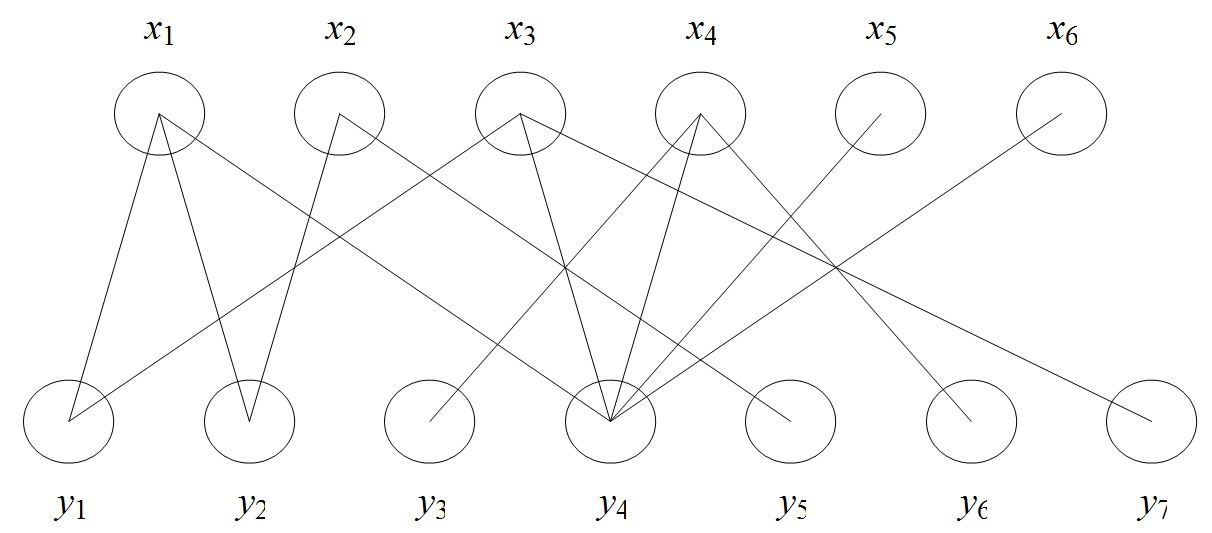
\includegraphics[scale=0.45]{p1.jpg}
\caption{初始二部图}
\end{figure}

\begin{figure}[htbp]%位置选项
\centering
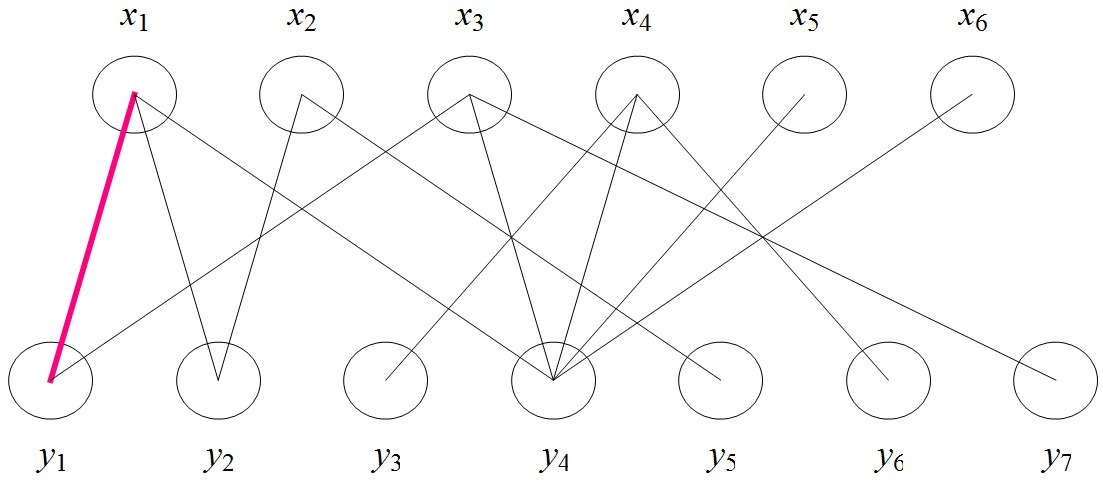
\includegraphics[scale=0.45]{p2.jpg}
\caption{从$x_1$开始找增广轨,直接找到$y_1$}
\end{figure}

\begin{figure}[htbp]%位置选项
\centering
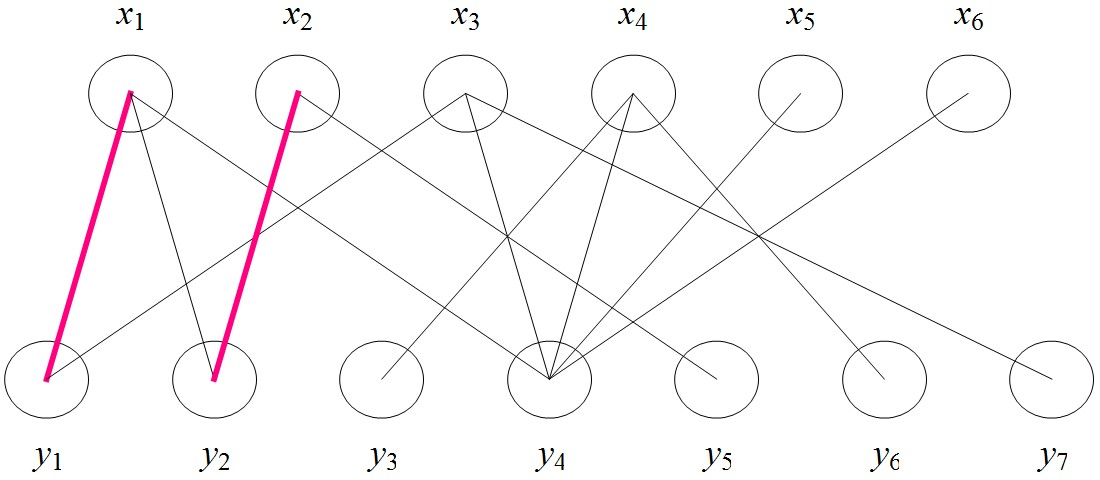
\includegraphics[scale=0.45]{p3.jpg}
\caption{从$x_2$开始找增广轨,直接找到$y_2$}
\end{figure}

\begin{figure}[htbp]%位置选项
\centering
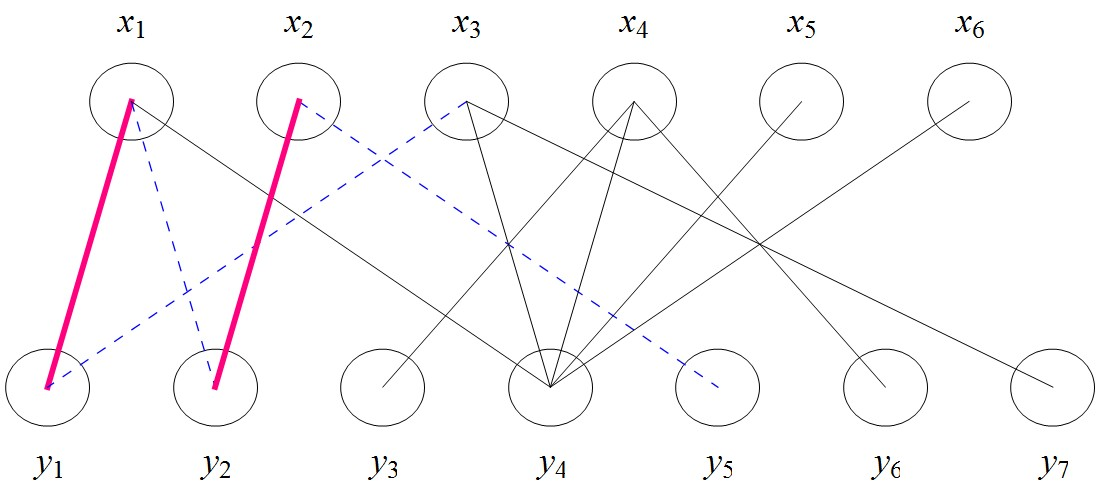
\includegraphics[scale=0.45]{p4.jpg}
\caption{从$x_3$开始找增广轨(蓝色虚线为增广轨)}
\end{figure}

\begin{figure}[htbp]%位置选项
\centering
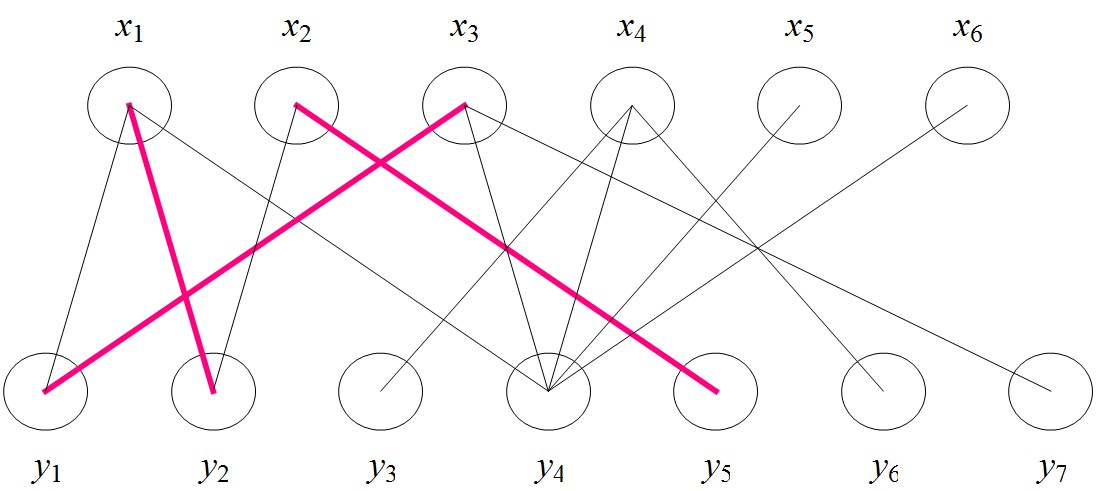
\includegraphics[scale=0.45]{p5.jpg}
\caption{更新最大匹配}
\end{figure}

\begin{figure}[htbp]%位置选项
\centering
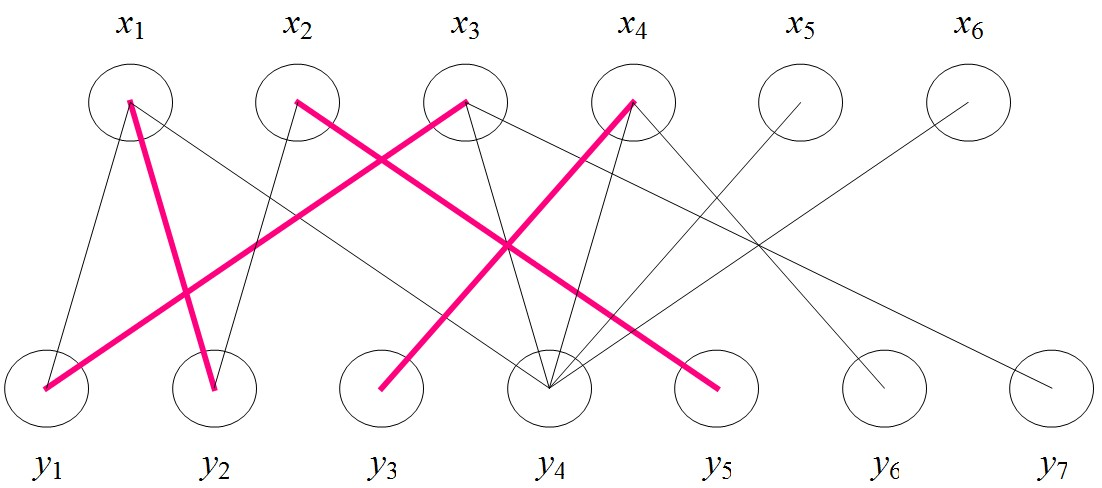
\includegraphics[scale=0.45]{p6.jpg}
\caption{从$x_4$找增广轨,直接找到$y_3$}
\end{figure}

\begin{figure}[htbp]%位置选项
\centering
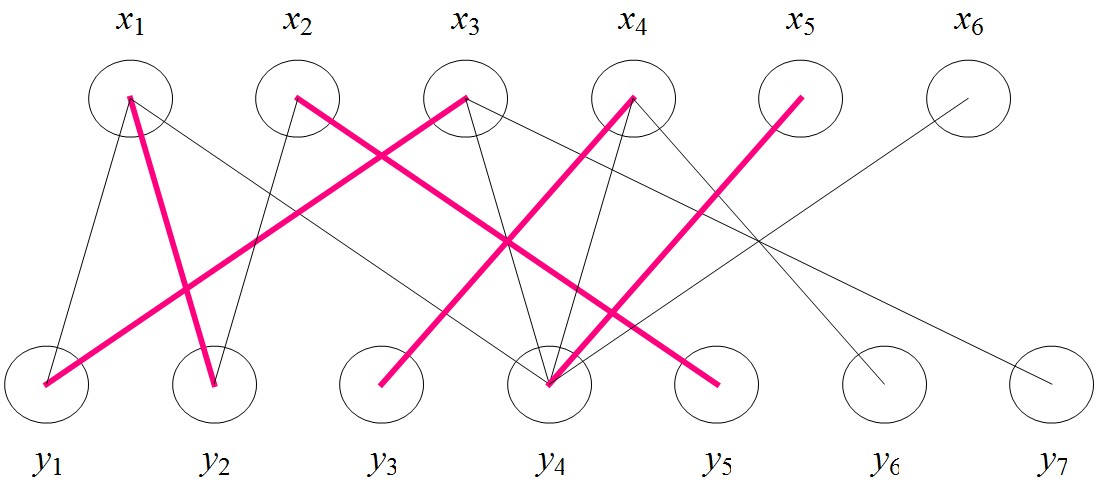
\includegraphics[scale=0.45]{p7.jpg}
\caption{从$x_5$找增广轨,直接找到$y_4$,从$x_6$找不到增广轨,结束.}
\end{figure}

\begin{figure}[htbp]%位置选项
\centering
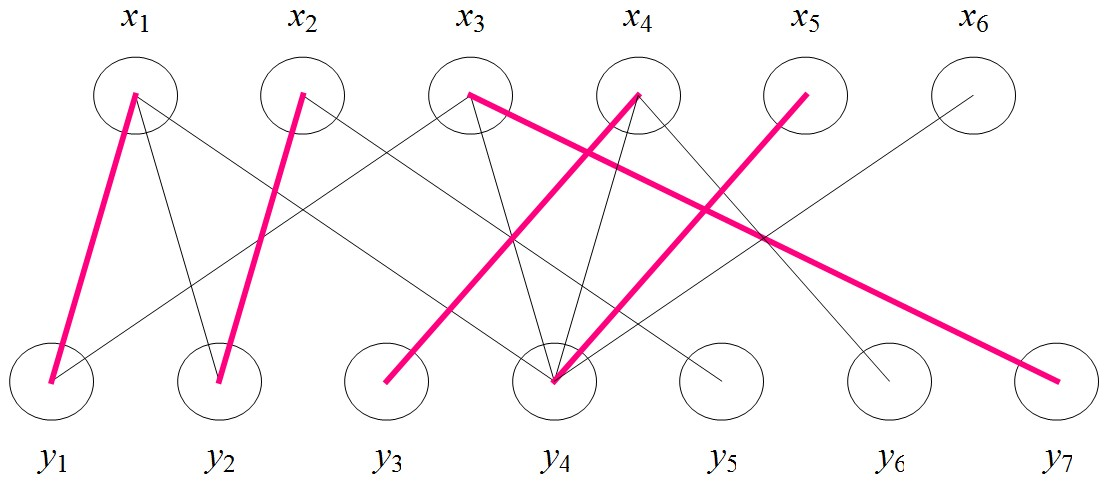
\includegraphics[scale=0.45]{p8.jpg}
\caption{另一个最大匹配}
\label{tu}
\end{figure}


二部图的最大匹配并不一定是唯一的,执行算法时遍历节点次序的不同可以得到不同的结果,比如图\ref{tu}也是一个最大匹配.

\chapter{算法实现与结果测试}

\section{主要功能函数}
\subsection{寻找增广轨}
adjl为邻接表,adjl[k][0]存储的是与k邻接的点的个数.
\begin{verbatim}
bool crosspath(int k)
{
    for (int i=1;i<=adjl[k][0];i++)
    {
        int j=adjl[k][i];//与k邻接的点
        if (!used[j])//若这个点不在增广轨上
        {
            used[j]=true;//那就把这个点加进增广轨
            if (mat[j]==0 || crosspath(mat[j]))
            //如果j是未被许配 或者 从j的对应项出发存在可增广轨(dfs)
            {
                mat[j]=k;//j与k匹配
                return true;
            }
        }
    }
    return false;
}
\end{verbatim}
\subsection{匈牙利算法}
\begin{verbatim}
void hungary()
{
    //遍历待未许配的顶点
    for (int i=1;i<=n;i++)
    {
        if (crosspath(i))//如果存在增广轨
            match++;//则匹配数增1
        memset(used,0,sizeof(used));//重置增广轨集合为空
    }
}
\end{verbatim}





\section{测试结果及分析}
加入适当的语句,我们可以看到算法的进行时状态的变化.可以看到在从3号节点开始找增广轨时有明显的回溯过程,因为这是一个深度优先搜索(DFS)
\centering
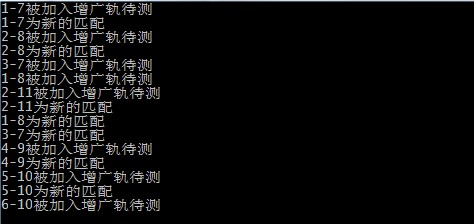
\includegraphics[scale=1]{p9.jpg}






\chapter{总结和问题}
\flushleft
  大二一年的学习,我们掌握了更多的编程的知识,也学习了更多的学科,这次的课题设计,不仅是不同学科之间的碰撞和交融,更是所学知识得以综合利用的一种体现,是自身综合能力的一次检验和锻炼,能有效的将所学的知识运用到实际,将不同的学科联系在一起,达到解决相关实际问题的目的。通过相关知识理论的了解和学习,终于设计出一种比较实际而又简洁的程序,很好的解决了二部图最大匹配问题。虽然这个计算程序已开发完成了,它也实现了我们所要解决的问题,但它仍有许多需要改进的地方。
\begin{enumerate}
	\item 无法求出所有的最大匹配.
	\item 无法针对特定的个体设计出满足其要求匹配的最大匹配,具有局限性.
\end{enumerate}



\begin{thebibliography}{123}
\bibitem{WSHlssxyl}
	王树禾. 离散数学引论 [M]. 合肥:中国科学技术大学出版社, 2001.
\bibitem{HFlssx}%洪帆离散数学
	洪帆. 离散数学基础(第三版)[M]. 武汉:华中科技大学出版社, 2011.
\end{thebibliography}
\acknowledgment
\hspace{\parindent}
  一份课程设计的总结,一份对老师的感谢。首先,必须感谢张晶老师的悉心教导和精心修改;过去的一学期,正是因为有像这样一批兢兢业业的老师,我们才可以在稳步的迈进程序设计的大门,正是由于他们的认真负责,我们才可以在这个贪玩的年龄里,在这个易受外物影响的年龄里能够很好的学到应该掌握的知识,能够很好的将学到的运用于实际;从而为走上社会,走上明天的岗位打好基础。
其次,必须感谢为了这份课程设计奉献过自己努力和给予帮助的同学,正是这份友谊,这份合作,我们才可以将这份课题设计圆满的完成,能够在这份设计中感受到友谊,同时也使自己得到相应的锻炼。
谢谢身边的每一个给予帮助的人,感谢生命中每一个孜孜奉献的每一个人,正是因为你们,所以我在这儿,健康而幸福的活着。
\clearpage
\phantomsection

\addcontentsline{toc}{chapter}{附录:程序代码}



\chapter*{附录:程序代码}
\begin{verbatim}

#include <iostream>
#include <cstdio>
#include <cstring>

#define MAX 100
using namespace std;
int n,n1,match;
int adjl[MAX][MAX];
int mat[MAX];
bool used[MAX];


bool crosspath(int k)
{
    for (int i = 1; i <= adjl[k][0]; i++)
    {
        int j = adjl[k][i];//与j邻接的点,一定属于另一个集合撒
        if (!used[j])//这个点不在增广路上
        {
            cout<<k<<"-"<<j<<"被加入交错路待测"<<endl;
            used[j] = true;//那就把这个点加进交错路
            if (mat[j] == 0 || crosspath(mat[j]))//如果j是未盖点 或者 从j的对应项出发存在增广路
            {
                mat[j] = k;
                cout<<k<<"-"<<j<<"为新的匹配"<<endl;
                return true;
            }
        }
    }
    return false;
}

void hungary()
{
    for (int i = 1; i <= n; i++)
    {
        if (crosspath(i))
            match++;
        memset(used,0,sizeof(used));//重置增广路集合为空
    }
}

int main()
{
    FILE *fi;
    fi = fopen("test.txt", "r");
    fscanf(fi, "%d%d", &n, &n1);
    long a,b;
    while (fscanf(fi,"%ld%ld",&a,&b) != EOF)
        adjl[a][++adjl[a][0]] = b;
    match  =0;

    hungary();
    cout<<"最大匹配数为:"<<match<<endl;
    return 0;
}
\end{verbatim}
\end{document}
